

PerfKit Benchmarker is an open source tool originally created at Google that allows users to easily run benchmarks on various cloud providers without having to manually set up the infrastructure required for those benchmarks. PerfKit Benchmarker follows the 5 step process detailed in Figure 1 to automate each benchmark run. The Configuration phase processes command line flags, configuration files, and benchmark defaults to establish the final specification used for the run. The Provisioning phase creates the networks, subnets, firewalls and firewall rules, virtual machines, drives, and other cloud resources required to run the test. Benchmark binaries and dependencies like datasets are also loaded in this phase. The Execution phase is responsible for running the benchmarks themselves,  and Teardown releases any resources created during the Provision phase. The Publishing phase packages the test results into a format suitable for further analysis such as  loading into a reporting system. The metadata returned from the Publishing phase can include verbose details about the actual infrastructure used during the test and timing information for each phase of the run along with the metrics returned from the benchmark itself, providing the level of detail needed to understand the benchmark results in context.


\begin{figure}[ht]
\centering
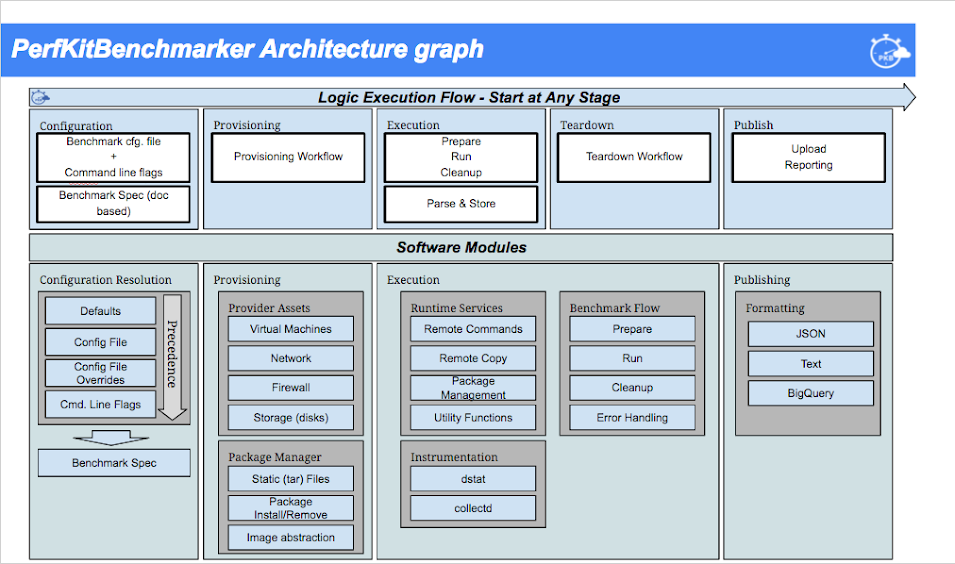
\includegraphics[width=.75\textwidth]{resource/img/ch_benchmarking/pkb_arch.png}
\caption{Perfkit Benchmarker Run Stage Breakdown}
\label{fig:benchmarking:pkb_arch}
\end{figure} 
